

\documentclass[conference]{IEEEtran}
%\usepackage {makecell}
\usepackage {url}
\usepackage {graphicx}
%\usepackage {caption}
\usepackage {algorithm}
\usepackage {algorithmic}
%\usepackage {algpseudocode}
\usepackage{amsmath}
\usepackage{tabu}
\usepackage[numbers,sort&compress]{natbib}
\usepackage{bbding}
% correct bad hyphenation here
\hyphenation{op-tical net-works semi-conduc-tor}

\begin{document}
% paper title
\title{Joint Energy-Aware and Buffer-Aided Relay Selection Strategy for Relay-Assisted D2D Communications}

% author names and affiliations
% use a multiple column layout for up to three different
% affiliations
\author{\IEEEauthorblockN{Lei Yu\IEEEauthorrefmark{1}, Xiaoxiang Wang\IEEEauthorrefmark{1}, Dongyu Wang\IEEEauthorrefmark{1}\Envelope}
\IEEEauthorblockA{\IEEEauthorrefmark{1}
 Key Lab. of Universal Wireless Comm., Ministry of Education, \\
 Beijing Univ. of Posts and Telecom., \\
 Beijing, P.R. China\\
Email(s): \{zzmikkz, cpwang, dy\_wang\}@bupt.edu.cn}}


% make the title area
\maketitle
% As a general rule, do not put math, special symbols or citations
% in the abstract
\begin{abstract}
Device-to-device (D2D) communication is a effective technique to improve performance on overall throughput and energy efficiency in cellular network. However, owing to the long separation distances or poor link quality between the source and destination user equipments (UEs), only using direct D2D communications limits the advantages of D2D communications. For enhancing traffic capacity in cellular network, relay-assisted D2D communications was proposed as a complement to direct D2D communications. The purpose of this work is to design a relay selection strategy that improve the D2D communication performance. In this paper, we propose an Energy-Aware and Buffer-Aided (EABA) relay selection scheme that considers several conditions jointly, including data rate, relay-available UE (RUE) residual energy, and RUE buffer state. Based on the channel states, energy, and buffer size, a scheduling rule is calculated dynamically by the EABA relay selection scheme at each time slot. And then, the scheduling rule specifies which of the source or relay nodes should use the channel for packet transmission. Simulation results validate the performance of the proposed scheme in terms of total amount of data transmitted and file transfer time under RUE residual energy and RUE buffer state.
\\
\textbf {\small \emph{Keywords --- Device-to-device communication, Relay selection, Limited energy, Buffer-Aided}}
\end{abstract}

\IEEEpeerreviewmaketitle
\section{Introduction}
% no \IEEEPARstart
To satisfy the increasing demand of local traffic load and provide better user experience, device-to-device (D2D) communications have been proposed for cellular network \cite{5350367,7949342,7254241}. D2D communications can be classified into licensed-band D2D and unlicensed-band D2D \cite{7128330}. Working on unlicensed bands is commonly subject to uncontrolled interference. Hence, most of the existing works focused on licensed-band D2D communications, aiming to improve spectrum efficiency and cell-wise data transmission performance by encouraging flexible radio resource reuse and communication mode selection \cite{7878672,7504380,7742334}.

However, most of the recent works have focused on direct D2D (one-hop D2D) communications. Only using direct D2D mode may limit the benefits brought in by the D2D communications to cellular network, because source and destination D2D-capable UEs (DUEs) may not be able to perform direct D2D communications due to long separation distance and poor channel condition between them \cite{7876267}. In such cases, a promising way to completely explore the benefits of D2D communications is to enable BS-controlled D2D transmission through relays, which can substantially extend the range of D2D communications \cite{7925800}.

Compared to fixed relay \cite{6775376}, the relay-capable UE (RUE) assisted D2D communications may be more flexible due to an increase in UE density. Hence, most works considered the "relays" in relay-involved D2D communications as RUEs. This paper focuses on the relay-assisted D2D, which works in the way that two DUEs within an BS's coverage communicate with each other, with the help of a relay-capable D2D UE under BS's control \cite{7450161,7752964}.

To develop relay-assisted D2D communications in cellular systems, the most critical issue is to select optimal relay UE for each D2D-capable communication pair in BS scheduling. Relay selection issues have been extensively studied in cooperative communications, ad hoc networks, and sensor networks. Most works assume that relaying procedure is performed in two consecutive time slots, where in the first slot, the source transmits to a relay and in the second slot, the relay forwards the received data to the destination. This relaying mechanism is referred to as conventional relaying \cite{6807959}. Moreover, most of the proposed relay selection strategies were designed in physical layer (PHY), the residual energy and buffer state of candidate relay node was basically ignored. Furthermore, the scenarios in most of these strategies did not include channel reuse.

In this paper, we treat relay-assisted D2D communication as a supplement to direct D2D communication in cellular systems, both of which should reuse the radio resources of general cellular UEs (CUEs). We propose a joint Energy-Aware and Buffer-Aided (EABA) relay selection strategy which uses the information about the channel conditions of the links, the residual energies and buffer states of the RUEs to compute a scheduling weight for each link at each time slot. The link with the highest weight is then selected to transmit data instead of conventional relaying \cite{7562509}.

The rest of this paper is organized as follows. We introduce a system model for relay-assisted D2D communications in cellular network and formulates optimization problems in Section \uppercase\expandafter{\romannumeral2}. A joint Energy-Aware and Buffer-Aided (EABA) relay selection strategy is proposed in Section \uppercase\expandafter{\romannumeral3}. The simulation results and analysis are presented in Section \uppercase\expandafter{\romannumeral4}, followed by the conclusions in Section \uppercase\expandafter{\romannumeral5}.

\section{System Model and Problem Formulation}
As shown in Fig. 1, we consider a network that consists of CUEs, RUEs, DUEs, which are all under the control of BS. We assume that there is only one pair of DUEs in the cell and presume that there are totally $M$ CUEs communicating with the BS via ordinary cellular uplinks. There are totally $N$ RUEs, which are idle cellular users and the candidate relay UEs that can be used to form relay-assisted D2D path. To simplify mathematical expressions in the following sections, let $C_{1},C_{2},\ldots,C_{i},\ldots,C_{M}$ denote $M$ CUEs, and $R_{1},R_{2},\ldots,R_{j},\ldots,R_{N}$ denote $N$ RUEs, i.e., $i\in\left[1,2,\ldots,M\right]$ and $j\in\left[1,2,\ldots,N\right]$. The two DUEs are denoted by $S$ and $D$, respectively, where the former is the source DUE and the later the destination DUE.
%Fig1
\begin{figure}[!t]
\center
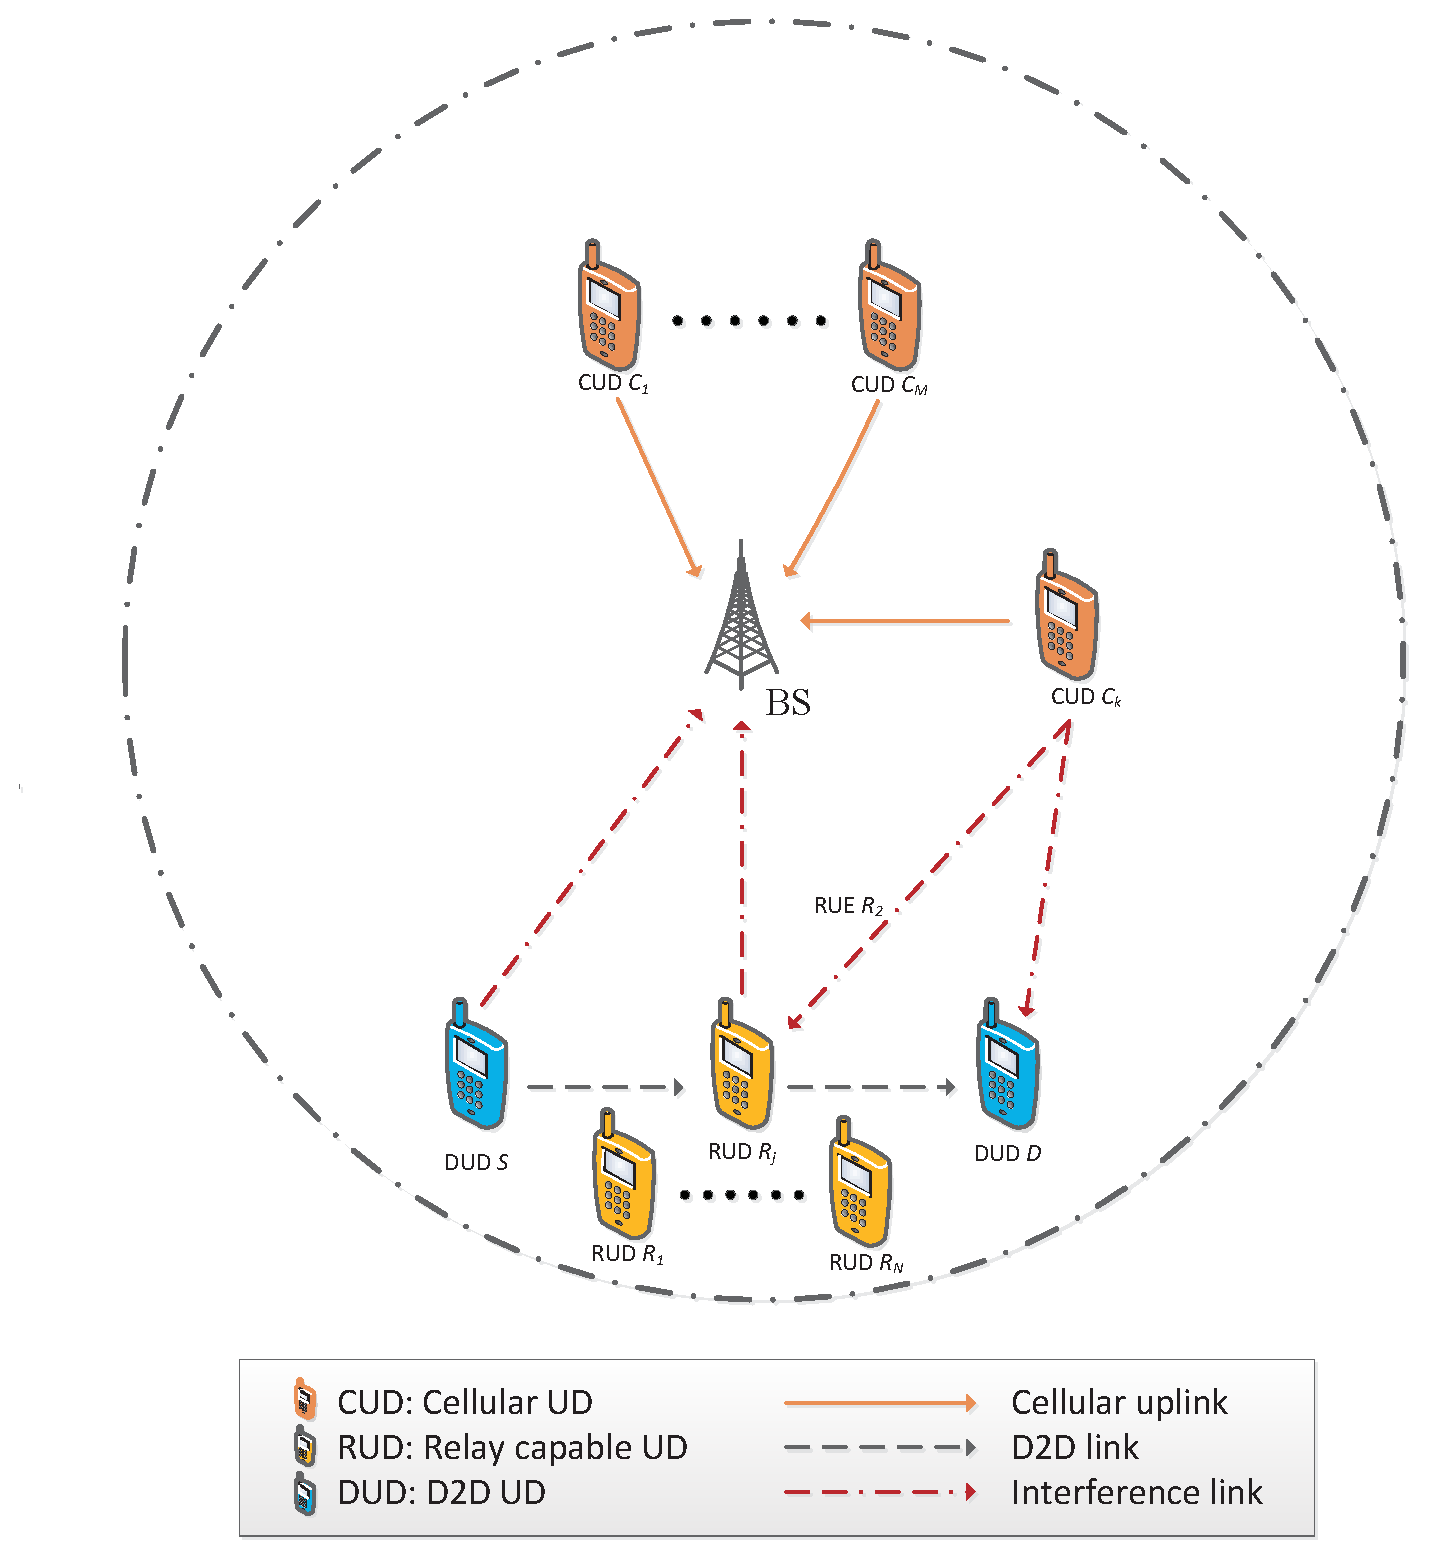
\includegraphics[width=3.5in]{fig1}
%where an .eps filename suffix will be assumed under latex,
% and a .pdf suffix will be assumed for pdflatex; or what has been declared
% via \DeclareGraphicsExtensions.
\caption{A single cell system model for D2D communications underlaying cellular architecture, in which uplink channel of CUE $C_k$ is reused by a D2D link. DUEs $S$ and $D$ are the source and destination D2D UEs, respectively. RUE $R_j$ is the selected relay UE for relay-assisted D2D communications.}
\label{fig_success}
\end{figure}

Furthermore, assume that $M$ CUEs are assigned $M$ separated cellular uplink channels by an BS. All channels have same bandwidth. Channel reuse is permitted for each of them. The D2D communication only reuse these uplink channels. Under these conditions,we consider the interference from potential reused CUEs to the relay UE and destination DUE and the interference from the source DUE and relay UE to the BS.

In addition, assume that the BS can obtain accurate channel state information (CSI) of all links. The BS is in charge of the entire cell and makes final decisions on D2D mode, relay UE, and reuse channel selection. We also assume that a minimum transmission quality should be met in terms of end-to-end signal to interference and noise ratio (SINR) for both cellular uplinks and D2D links.

We consider a channel model between two UEs or between a UE and the BS as follows \cite{6560489} :
\begin{equation}
|{h_{a,b}}|^{2} = K_{0}\beta_{a,b}\zeta_{a,b}\cdot L_{a,b}^{-\alpha}
\end{equation}
in which path loss, slow fading, and fast fading are taken into account. $|{h_{a,b}}|^{2}$ is the channel gain from transmitter $a$ to receiver $b$. $K_{0}$ is a constant corresponding to the path loss model. $\beta_{a,b}$ and $\zeta_{a,b}$ denote slow and fast fading gains, respectively. The slow fading is usually log-normally distributed and fast fading is exponentially distributed. $L_{a,b}$ is the distance between $a$ and $b$. $\alpha$ is the path loss exponent.

The goal of this paper is to efficiently utilize the energy resources of the nodes as well as time and space diversity to minimize the transfer time of a file with $Q$ packets, from the source to the destination before the network becomes unavailable. Let $T\left(\chi\right)$ denote the file transfer time achieved with strategy $\chi$, i.e., the time interval since packet $1$ is transmitted at the source node until packet $N$ is received at the destination node, the problem can be stated as
\begin{align}
&\displaystyle \min _{\mathcal {\chi}} ~T(\mathcal {\chi})
\\[-5pt]&\text {subject to} ~ \sum T_{j} \leq \tau_j(1) , \quad \forall j , \tag{2a}
\\[-1.5pt]&\qquad \qquad ~ j\in\left[1,2,\ldots,N\right] , \tag{2b}
\end{align}
where $\sum T_{j}$ denote RUE $R_{j}$ total working time, and $ \tau_j(1)$ denote the residual work time of relay $R_j$ in time slot 1.

\section{EABA Relay Selection Strategy}
As mentioned earlier, the BS needs to select an optimal links according to end-to-end data rate, RUE residual energies and RUE buffer states. Hence, in this section, we demonstrate the methods of estimation of the end-to-end data rates of the links between DUEs and RUEs, the residual energies and buffer states of RUEs. We will also propose a relay selection strategy to address the problem in Section \uppercase\expandafter{\romannumeral2}.

\subsection{Link Data Rate Estimation}
As shown in Fig. 1, the link data rate is derived in this subsection. Let $P_{C_i},P_S$, and $P_{R_j}$ represent the transmit power of the CUE $C_i$, the source DUE, and RUE $R_j$, respectively. In addition, we assume that the noise $n_0$ at each receiver UE is additive white Gaussian noise (AWGN) with zero mean and variance $\sigma^2$, i.e., $n_0 \sim (0,\sigma^2)$. RUE $R_j$ is assumed to work on half-duplex mode. If link $S \rightarrow R_j$ is selected as a transmission link and the uplink channel of $C_i$ $(i \in [1,2,\ldots,M])$ is selected as the reuse channel, the received signal at $R_j$ can be expressed as
\begin{equation}
y^i_{S,R_j} = h_{S,R_j}\cdot x_S + h_{C_i,R_j}\cdot x_{C_i} + n_0
\end{equation}
where $x_S$ is the signal transmitted from the source DUE $S$, $h_{C_i,R_j}\cdot x_{C_i}$ denote the received interference from CUE $C_i$ at $R_j$. If link $R_j \rightarrow D$ is selected as a transmission link and the uplink channel of $C_k$ $(k \in [1,2,\ldots,M])$ is selected as the reuse channel, the received signal at destination DUE $D$ can be expressed as
\begin{equation}
y^k_{R_j,D} = h_{R_j,D}\cdot x_{R_j} + h_{C_k,D}\cdot x_{C_k} + n_0
\end{equation}
where $x_S$ is the signal transmitted from $R_j$, $h_{C_k,D}\cdot x_{C_k}$ denote the received interference from CUE $C_k$ at destination DUE $D$.

The corresponding SINR at $R_j$ and destination DUE $D$ are
\begin{equation}
\gamma^{i}_{S,R_j} = \frac{P_S|{h_{S,R_j}}|^{2}}{P_{C_i}|{h_{C_i,R_j}}|^{2} + \sigma^2} ,\gamma^{k}_{R_j,D} = \frac{P_{R_j}|{h_{R_j,D}}|^{2}}{P_{C_k}|{h_{C_k,D}}|^{2} + \sigma^2}
\end{equation}
respectively. The achievable data rate of link $S \rightarrow R_j$ and $R_j \rightarrow D$ can be expressed as
\begin{equation}
R_{S,R_j} = B\log_2(1 + \gamma^{i}_{S,R_{j}}),R_{R_j,D} = B\log_2(1 + \gamma^{k}_{R_j,D})
\end{equation}
respectively, where $B$ is channel bandwidth.

Similarly, for the reused cellular uplink channel, SINR at the BS is
\begin{equation}
\gamma^{j}_{C_i,B} = \frac{P_{C_i}|{h_{C_i,B}}|^{2}}{P_S|{h_{S,B}}|^{2} + \sigma^2} ,\gamma^{j}_{C_k,B} = \frac{P_{C_k}|{h_{C_k,D}}|^{2}}{P_{R_j}|{h_{R_j,B}}|^{2} + \sigma^2}
\end{equation}
respectively, where B in the subscripts denote BS.

\subsection{RUE Residual Energy And Buffer State Estimation}
Note that due to the limited energies of the relays, each relay can transmit a limited number of packets before it runs out of energy. Hence, even if a relay has enough space in its buffer, there is no point in sending more packets to it than it can forward later. To take this into account,we should know the data size can be transmitted of RUE $R_i$ under the residual energy.

Let $E_{1},E_{2},\ldots,E_{j},\ldots,E_{N}$ denote the total energies of $N$ RUEs, respectively. To capture the relationship between remaining operation time and transmit power for each RUE, an empirical mode, i.e., Peukert's Law \cite{6981957}, is adopted here as
\begin{equation}
\tau_j = E_j/I^{\alpha}_j
\end{equation}
where $\tau_j$ denotes the remain operation time of $R_j$ with a transmit power $P_{R_j}$, $I_j$ is discharge current, and $\alpha$ is a constant to indicate the non-linear effect and its value is around 1.3 \cite{6981957}. Assume that if transmit power of $R_j$ is $P_{R_j}$, the discharge current can be expressed by discharge voltage and total power consumed, i.e., $I_j = P_{R_j} / V_0$, where $V_0$ denote the discharge voltage of each UE. Without loss of generality, we assume the same $V_0$ for all UEs.

Hence, if residual energy, transmit power, and discharge voltage are known for each RUE, the remaining operation time can be estimated. In this paper, the transmit power of all UEs are predefined as a fixed value, so we can use the remaining operation time $\tau_j$ denotes the residual energy of RUE $R_j$. Then the minimum data size can be transmitted of RUE $R_j$ can be expressed as
\begin{equation}
\theta_j = R_{min} \cdot \tau_j
\end{equation}
where $R_{min}$ is the minimum transmission speed of RUE $R_j$.
%Fig2
\begin{figure}[!t]
\center
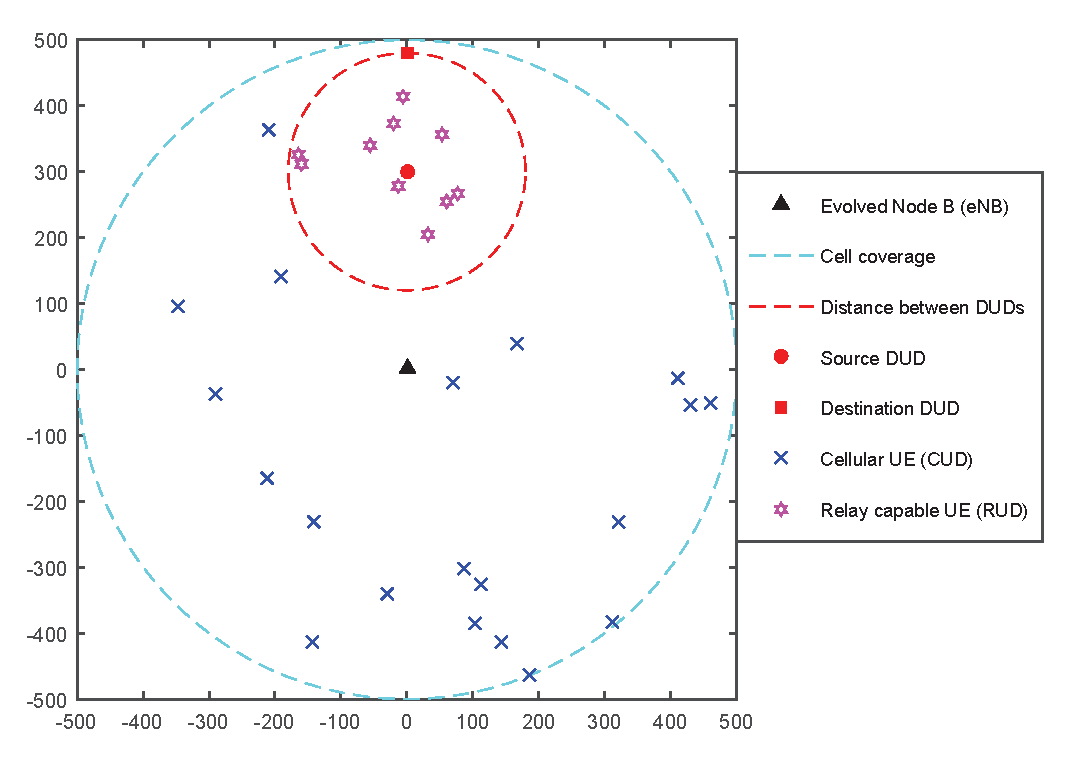
\includegraphics[width=3.5in]{fig2}
%where an .eps filename suffix will be assumed under latex,
% and a .pdf suffix will be assumed for pdflatex; or what has been declared
% via \DeclareGraphicsExtensions.
\caption{Simulation scenario for the proposed relay selection scheme, where the numbers of CUEs and RUEs are 20 and 10, respectively. The distance between the source and destination DUEs is 220m.}
\label{fig_scenario}
\end{figure}
Without loss of generality, we assume that a time slot is of unit duration, and therefore if a relay transmits in a slot, its residual energy is reduced by the amount of its transmission time, e.g., $\tau_j(t+1) = \tau_j(t) - tran_j(t)$, where $tran_j(t)$ denotes the transmission time of RUE $R_j$ to the destination. Let $Q_j(t)$ denote the number of packets stored in the buffer of RUE $R_j$ at the beginning of time slot $t$, and $e_j(t) = L_j -  Q_j(t)$, where $L_j$ denotes the total buffer size of RUE $R_j$, so $e_j(t)$ is the buffer size of RUE $R_j$ can be used at the beginning of time slot $t$. And then, the $tran_j(t)$ can be expressed as
\begin{equation}
tran_j(t) = \begin{cases}T & R_{R_j,D}(t)\cdot T \leq Q_j(t)\\Q_j(t)/R_{R_j,D}(t) & R_{R_j,D}(t)\cdot T > Q_j(t)\end{cases}
\end{equation}
where $T$ is duration of a time slot, and $R_{R_j,D}(t)$ is the data rate of link $R_j \rightarrow D$ at time slot $t$.

\subsection{EABA Strategy}
In order to transfer the packets of a file in a short period of time, Energy-Aware and Buffer-Aided (EABA) works based on the following theory based: if a relay has high residual energy and many empty spaces in its buffer, it should get a higher chance for reception. On the other hand, if it has a large number of data in its buffer, it should have a higher chance for transmitting a packet to the destination. Moreover, if a link has a high SINR, more data will be transmitted at a time slot, it should get a higher priority.

In the EABA strategy, relay $R_j$ computes the weight for its incoming link as
\begin{equation}
W_{S\rightarrow R_j} = min(\theta_j - Q_j,e_j) \cdot R_{S\rightarrow R_j} \cdot I[\gamma_{S\rightarrow R_j} \geq \gamma_d)]
\end{equation}
where $I[x]$ is the indicator function, which is 1 if x is true and zero otherwise. Thus, a link $S \rightarrow R_j$ get a positive weight only if relay $R_j$ has enough buffer space and residual energy, and the link SINR must no less than the predefined SINR requirement for D2D link.

Similarly, for its outgoing link, relay $R_j$ computes the weight as
\begin{equation}
W_{R_j \rightarrow D} = Q_j \cdot R_{R_j \rightarrow D} \cdot I[\gamma_{R_j \rightarrow D} \geq \gamma_d)]
\end{equation}
According to (12), a link $R_j \rightarrow D$ get a positive weight only if relay $R_j$ has data stored in its buffer, and the link SINR must not less than the predefined SINR requirement for D2D link.

After computing the weights according to EABA strategy, the link $l^*$ from among all the $S \rightarrow R_j$ and $R_j \rightarrow D$ links is activated, where
\begin{equation}
l^* = \arg \max_{l \in \{S \rightarrow R_j\} \cup \{R_j \rightarrow D\}}\{W_l\}
\end{equation}

\begin{algorithm}[!t]
\caption{EABA Relay Selection Strategy}
\begin{algorithmic} [1]
\STATE {Each relay computes the minimum data size can be transmitted using (9).}
\STATE{Each relay computes the weight for its incoming link using (11).}
\STATE{Each relay computes the weight for its outgoing link using (12).}
\STATE {In a distributed way, the best link is selected based on (13).}
\end{algorithmic}
\end{algorithm}

Algorithm 1 summarizes all the steps of the EABA scheme. Note that the EABA strategy is based on the local information about the channel states, residual energy and buffer size in each relay. Therefore, it can be implemented in a distributed way similar to the \emph{opportunistic carrier sensing} technique proposed in a previous study \cite{4244758}. Specifically, the timer of the relay with the highest weight will expire first. That relay will broadcast a flag packet signaling its priority to other relays and notifying whether the source should transmit to it or the relay itself will transmit.

The above procedure continues as long as the network is operable. According to the earlier discussion about the EABA scheme, if there are some data in the buffer of $R_j$, $R_j$ will have enough energy to transmit that data. Considering that the probability of having a good channel condition for link $R_j \rightarrow D$ is non-zero, there will be a time slot in the future in which that data will be transmitted by $R_j$ and received successfully at the destination. Therefore, when the network becomes inoperable, there will be no data remaining in the buffer of relay $R_j$.

\section{Simulation Results}
In this section, the proposed relay selection scheme is evaluated via simulations in MATLAB. The scenario is a single cell with its radius equal to 500 meters. All CUEs are random distributed in the cell. There are only two DUEs to perfom D2D communication, i.e., the source and destination. All RUEs are random distributed in a circular area with the source DUE as its center. Fig. 2 shows the scenario, and Table \uppercase\expandafter{\romannumeral1} lists primary parameters used therein. Note that all UEs are re-deployed random according to the defined conditions in different experiments, and the same scenario was tested for 100,000 times to get an average value.
%Table 1
\begin{table}[!t]
  \centering
  \scriptsize
  \caption{Simulation parameters}
  \label{tab:notations}
  \begin{tabular}{m{3cm}m{3cm}}
    \\[-2mm]
    \hline\\[-2mm]
    {\bf  Parameters}& {\bf Value}\\
    \hline
    \hline
    \vspace{1mm}\\[-3mm]
    Cell radius      &    500 m\\
    \hline
    \vspace{1mm}\\[-3mm]
    Noise power spectral density &    -174 dBm/Hz \\
    \hline
    \vspace{1mm}\\[-3mm]
    Transmit power of UEs &  24 dBm\\
    \hline
    \vspace{1mm}\\[-3mm]
    Path loss exponent ($\alpha$) &  4 \\
    \hline
    \vspace{1mm}\\[-3mm]
    Path loss constant ($K_0$) &   0.01\\
    \hline
    \vspace{1mm}\\[-3mm]
    SINR requirements for cellular and D2D links ($\gamma_c,\gamma_d$) &  20 dB \\
    \hline
    \vspace{1mm}\\[-3mm]
    Slow fading coefficient ($\beta_{a,b}$) &  Log-normal distrubution with standard deviation of 8 dB and zero mean\\
    \hline
    \vspace{1mm}\\[-3mm]
    Fast fading coefficient ($\zeta_{a,b}$) &  Exponential distribution with unit mean\\
    \hline
    \vspace{1mm}\\[-3mm]
    Number of packet in source DUE &  50 \\
    \hline
    \vspace{1mm}\\[-3mm]
    Number of data bits in a packet &  1024 bits\\
    \hline
    \vspace{1mm}\\[-3mm]
    Duration of a time slot ($\triangle T$) &  $1 \mu s$\\
    \hline
    \vspace{1mm}\\[-3mm]
    RUE total energy ($E_i$) &  Randomly distributed in [0,1440] mAh \\
    \hline
  \end{tabular}
\end{table}

The proposed relay selection scheme, considering end-to-end data rate, RUE residual energy and RUE buffer state, is validated by the simulations as shown in Fig. 3, 4, 5. To evaluate the necessity of the proposed relay selection scheme, "random relay selection", "rate based relay selection" and "EABA relay selection" are compared. In "random relay selection", the BS just select a link randomly from link $S\rightarrow R_j$ and link $R_j\rightarrow D$; in "rate based relay selection", the BS will select a link has maximum SINR, i.e., the maximum transfer rate, from link $S\rightarrow R_j$ and $R_j\rightarrow D$; whereas in the "EABA relay selection", the BS will select the optimal link in the evaluation process which is proposed in Section \uppercase\expandafter{\romannumeral3}. All the three relay selection schemes assume that direct D2D mode is unavailable. The three schemes are only working in relay-assisted D2D mode. In addition, we also ignore the time and energy consumption caused by  calculation.

%Fig3
\begin{figure}[!t]
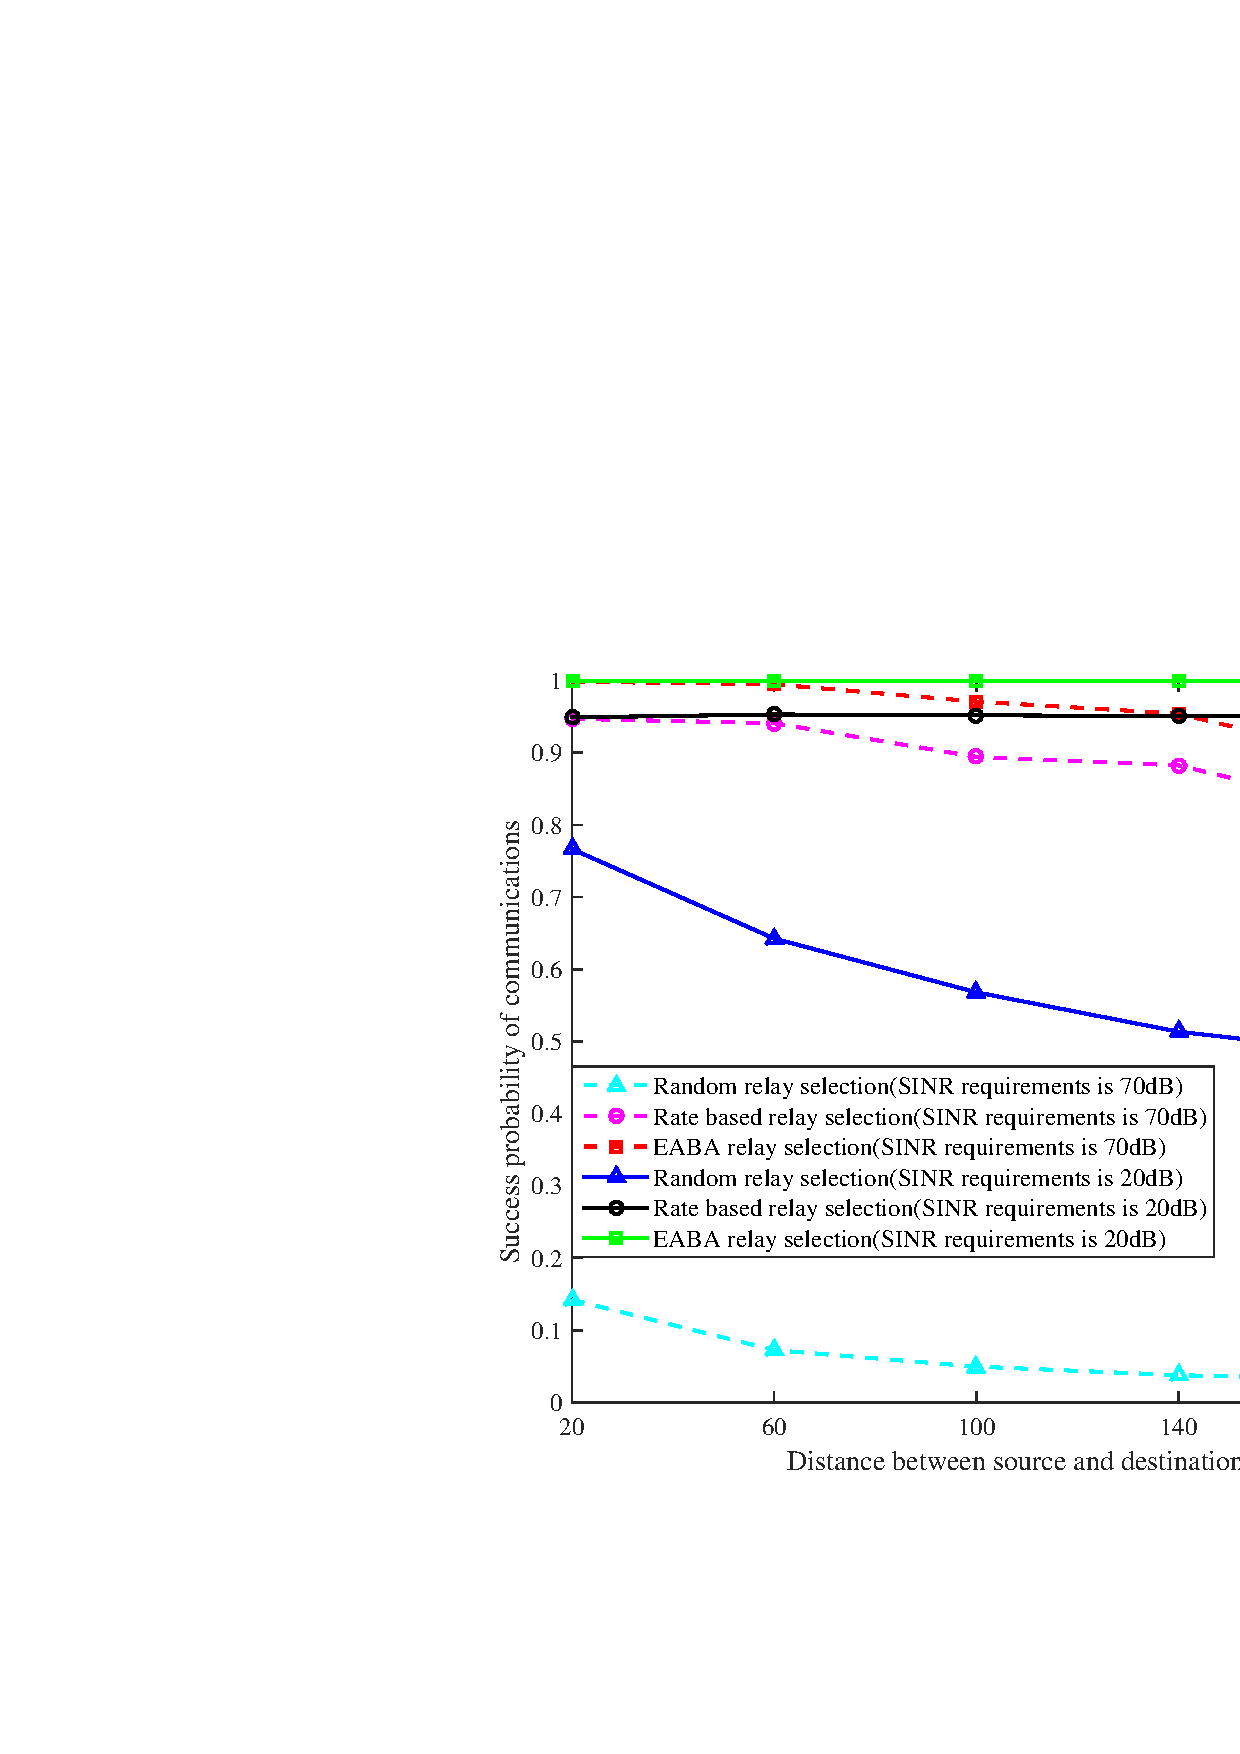
\includegraphics[width=3.5in]{fig3.pdf}
%where an .eps filename suffix will be assumed under latex,
% and a .pdf suffix will be assumed for pdflatex; or what has been declared
% via \DeclareGraphicsExtensions.
\caption{Success probability for D2D communications with varying distances between source and destination DUEs under different relay selection strategies, where the number of CUEs and RUEs are 20 and 10, respectively. The buffer size at each UE is 5, the bandwidth of each channel is 720 kHz.}
\label{fig_success}
\end{figure}
%Fig4
\begin{figure}[!t]
\center
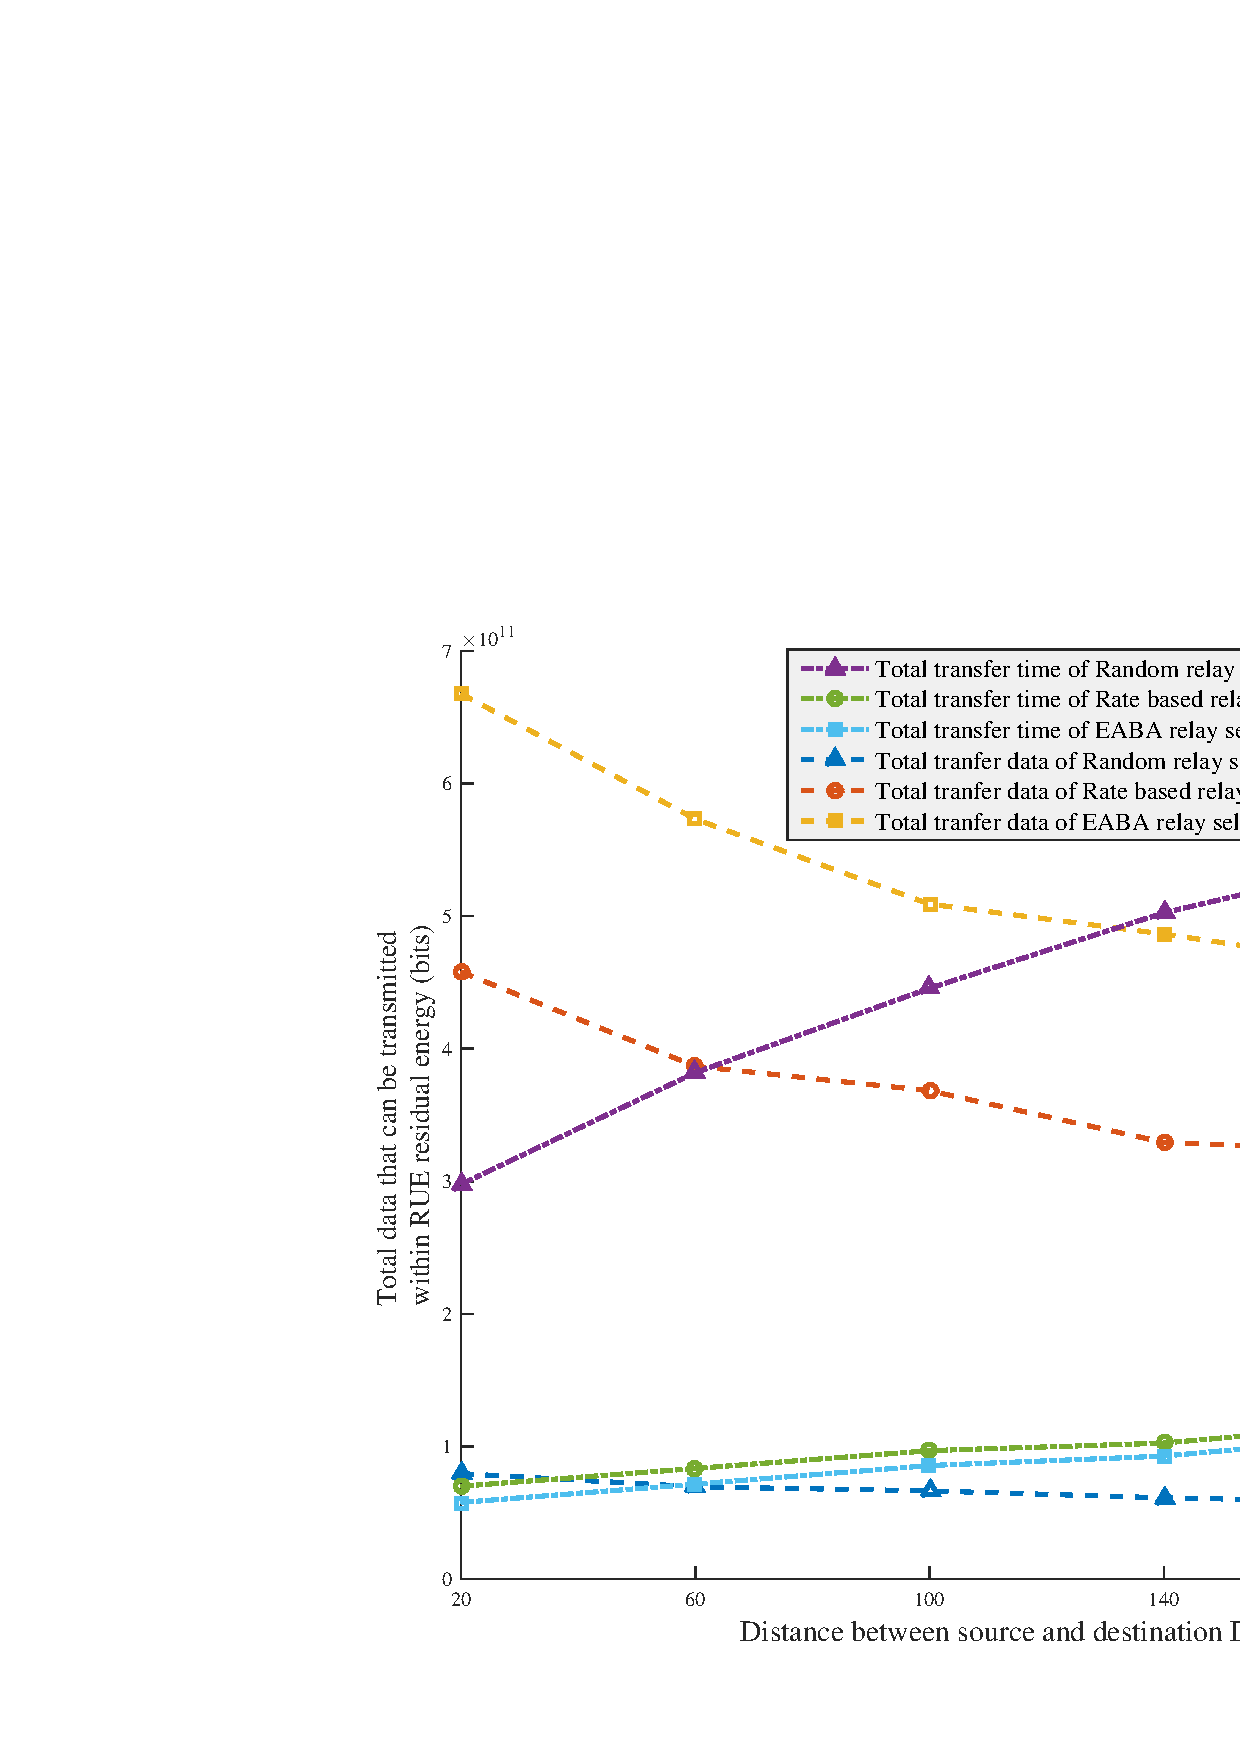
\includegraphics[width=3.5in]{fig4.pdf}
%where an .eps filename suffix will be assumed under latex,
% and a .pdf suffix will be assumed for pdflatex; or what has been declared
% via \DeclareGraphicsExtensions.
\caption{Total data amount transmitted within RUE residual energy and total transmission time with varying distances between source and destination DUEs under different relay selection strategies, where the number of CUEs and RUEs are 20 and 10, respectively. The buffer size at each UE is 5, the bandwidth of each channel is 720 kHz.}
\label{fig_time}
\end{figure}

It is seen from Fig. 3 that the probability of successful communications using random relay selection, rate based relay selection and EABA relay selection decreases as the distance between DUEs $S$ and $D$ increases. This is reasonable, as the average distance between random distributed RUEs and DUEs will increase with the increasing distance between DUEs $S$ and $D$. So the channel gain for link between DUEs and RUEs will decrease with an increasing separation, which will reduce the success probability of D2D communication. Specifically, the strategy based on EABA relay selection presents the best performance on the success probability. The reason is that random relay selection strategy randomly selects a link, SINR of which may not meet the requirements for D2D links and subsequently lead to communication failure. And rate based relay selection strategy selects a link has maximum end-to-end data rate, but the RUEs buffer states and residual energies are not considered. So the strategy to select a link from $S$ to RUE with maximum end-to-end data rate, but the RUE does not have enough buffer space or residual energy which may lead to communication failure. Furthermore, no matter which strategy is used, a lower link SINR requirement results in higher success probability of D2D communications.

Fig. 4 shows that the total data transmission time of the three relay selection strategies become worse off as the distance between $S$ and $D$ is enlarged. The reason is that enlarging separation distance may reduce data rate on both source-to-relay and relay-to-destination links. Reducing data rate means that servicing rate is decreased, directly leading to a decreased data transmission in both of the links. Thus, the total data transmission time will increase. In the three strategies, the EAPA strategy has the minimum total transfer time, because it has a higher data rate and communications success probability. The random relay selection strategy shows the worst performance, due to its lowest link data rate and communications success probability. Although rate based relay selection strategy select the fastest link, but the lower communication success probability than EABA strategy leading to an higher transmission time than EABA strategy.
%Fig5
\begin{figure}[!t]
\center
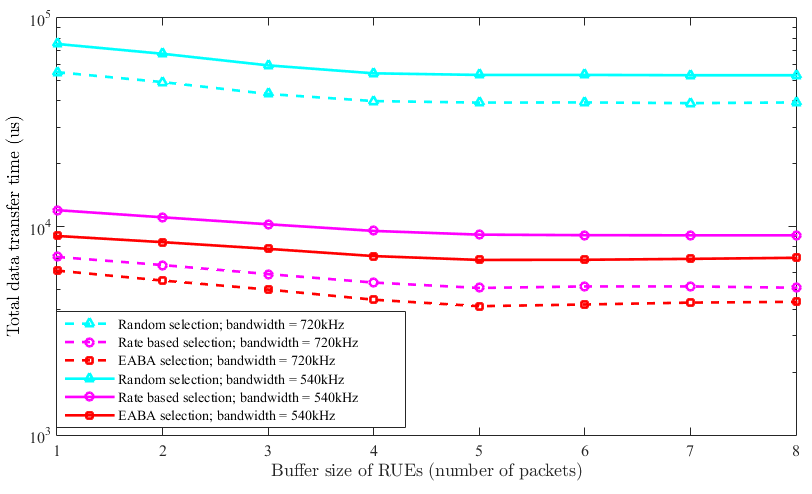
\includegraphics[width=3.5in]{fig5.pdf}
%where an .eps filename suffix will be assumed under latex,
% and a .pdf suffix will be assumed for pdflatex; or what has been declared
% via \DeclareGraphicsExtensions.
\caption{Total data amount transmitted within varying buffer size, and different relay selection strategies and channel bandwidths, where the distance between source and destination DUEs is 180m, where the number of CUEs and RUEs are 20 and 10, respectively.}
\label{fig_time}
\end{figure}

Fig. 4 shows that the total amount of data transmitted within RUE residual energy with varying distances between DUEs $S$ and $D$ using three relay selection strategies. The performance on total data amount under three strategies degrades with an increasing separation distance. Increasing separation distance will increase path loss, resulting in a decreasing link data rate. In addition, with the same system parameters, the random strategy offers a much worse performance on total data amount than the other two selection strategies, because the selected link data rate and residual energy of RUE is not considered in the relay selection. Although rate based strategy gives the highest link data rate, it can only work for a very short period of time, due to the fact that residual energy of RUE is not considered in the relay selection, leading to a smaller amount of data transmitted than EABA strategy. The EABA strategy gives the best performance on total data amount, because it not only ensure the system work more time, but also ensure the link data rate.

Fig. 5 illustrates the influences of RUE's buffer size on the total data transmission time with the three relay selection strategies and different channel bandwidths. Given a bandwidth and a relay selection strategy, if buffer size is less than 5, increasing the buffer size of RUEs leads to a decrease in the total data transmission time. As the buffer size increases, the probability of successful communications increases, and this leads to lower total data transmission time. Otherwise, the total time isn't influenced by buffer size when it is greater than 5. The reason is that the communication failure caused due to RUEs lack of buffer size which does not happen when RUEs has enough buffer size. No matter which strategy is used, reducing channel bandwidth will dramatically increase the total data transmission time. Because a smaller bandwidth leads to a lower data rate on each link. In addition, with the same buffer size and channel bandwidth, the total data transmission time of EABA strategy is better than that of the random and rate based strategies, and the advantage becomes more evident if the bandwidth is relatively small.

\section{Conclusion}
In this paper, we designed an efficient relay selection scheme for Relay-Assisted D2D communication in cellular network. Under the assumption that D2D communication reuse the uplink channels of CUEs, we proposed a Energy-Aware and Buffer-Aided (EABA) relay selection scheme, which jointly considered end-to-end data rate, RUEs residual energies, and RUEs buffer states. The estimation processes of the end-to-end data rate, RUEs residual energies, and RUEs buffer states were described. Specially, we established a relay selection scheme which select the best link instead of selecting best relay. Simulation results showed that the proposed scheme provides the best overall transmission performance compared to other relay selection schemes,.

\section*{Acknowledgment}
This work was supported by the National Key Technology R\&D Program (No.2015BAI01B14) and the Fundamental Research Funds for the Central Universities.
% references section
% trigger a \newpage just before the given reference
% number - used to balance the columns on the last page
% adjust value as needed - may need to be readjusted if
% the document is modified later
\bibliographystyle{IEEEtran}
\bibliography{ref}

\end{document} 